\section{Cas d'un objet plan infini}
    % Ce cas est très bien documenté (\cite{senior_approximate_x995},\cite{hoppe_impedance_x995}) et pose la méthodologie à adopter pour les objets courbes.

    \begin{figure}[!h]
        \begin{center}
            \begin{tikzpicture}
                \tikzmath{
    \largeur = 6;
    \hauteur = 1;
    \milieu = 1.3;
    \xC = \largeur;
    \xA = 0;
}

%% 1ere couche
\tikzmath{
    \yC = \hauteur;
    \yA = 0;
}

\coordinate (A) at (\xA,\yA);
\coordinate (B) at (\xA,\yC);
\coordinate (C) at (\xC,\yC);

\draw ($(B)!0.5!(C)$) node [above] {vide};


\fill [lightgray] (A) rectangle (C);
\draw ($(A)!0.5!(C)$) node {$\peps,\pmu,d$};
\draw (B) -- (C) node [right] {$\z = 0$};

%% Le repère
\tikzmath{
    \xD = \xC + 1.5;
}

\coordinate (n) at (\xD,\yA);

\draw [->] (n) -- ++(0,1) node [at end, right] {$\v{\z}$};
\draw [->] (n) -- ++(1,0) node [at end, right] {$\v{\x}$};

\draw (n) circle(0.1cm) node [below=0.1cm] {$\v{\y}$};
\draw (n) +(135:0.1cm) -- +(315:0.1cm);
\draw (n) +(45:0.1cm) -- +(225:0.1cm);

%% Le conducteur
\tikzmath{
    \yC = \yC - \hauteur;
    \yA = \yA - 0.5*\hauteur;
}

\coordinate (A) at (\xA,\yA);
\coordinate (B) at (\xA,\yC);
\coordinate (C) at (\xC,\yC);
\draw (B) -- (C);

\fill [pattern=north east lines] (A) rectangle (C);



            \end{tikzpicture}
        \end{center}
    \end{figure}

    Dans un premier temps, on peut sans perte de généralités faire une rotation du repère pour avoir le plan orthogonal à \(\vect{z}\). Comme il est infini dans les directions \(\vect{e_x} \vect{e_y}\) et que le matériau est homogène isotrope, on utilise la transformée partielle en \(x, y\) seulement.
    \begin{equation}
        \vE(x,y,z) = \frac{1}{2\pi}\iint_{\RR^2} e^{i(k_x x + k_y y)}\hat{\vE} (k_x,k_y,z) \dd{k_x}\dd{k_y}
    \end{equation}

    \begin{prop}
        Soient \(\vect{X}(k_x,k_z,z) =
        \begin{bmatrix}
        \hat{E_x} &
        \hat{E_y} &
        \hat{H_x} &
        \hat{H_y}
        \end{bmatrix}^t\),
        où \((\hat \vE,\hat \vH)\) sont des solutions du problème \eqref{eq:imp_fourier:intro:maxwell_harmonique}, alors il existe une matrice \(\mat{M}\) ne dépendant pas de \(z\) telle que
        \begin{equation}
            \ddr{z}{}\vect{X}(k_x,k_z,z) = \mat{M}(k_x,k_z) \vect{X}(k_x,k_z,z)
            \label{eq:imp_fourier:plan:edo}
        \end{equation}
    \end{prop}

    \begin{proof}
        En utilisant les multiplicateur de Fourier associés aux opérateurs différentiels, le problème \eqref{eq:imp_fourier:intro:maxwell_harmonique} s'écrit
        \begin{align*}
            \left\lbrace
            \begin{matrix}
            ik_y \hat{E_z}  - \ddr{z}{\hat{E_y}} = -i \w \mu \hat{H_x} \\
            \ddr{z}{\hat{E_x}} - ik_x \hat{E_z} = -i\w \mu \hat{H_y} \\
            ik_x \hat{E_y} - ik_y \hat{E_x} = -i\w \mu \hat{H_z} \\
            \end{matrix}
            \right. \quad
            \left\lbrace
            \begin{matrix}
            ik_y \hat{H_z}  - \ddr{z}{\hat{H_y}} = i \w \eps \hat{E_x} \\
            \ddr{z}{\hat{H_x}} - ik_x \hat{H_z} = i\w \eps \hat{E_y} \\
            ik_x \hat{H_y} - ik_y \hat{H_x} = i\w \eps \hat{E_z} \\
            \end{matrix}
            \right.
        \end{align*}

        Les composantes normales se déduisant des composantes tangentielles, on résout l'équation différentielle  matricielle à coefficients constants
        suivante \(\ddr{z}{}\vect{X} = \mat{M} \vect{X}\) où

        \begin{equation}
            \mat{M} = \begin{bmatrix}
            0 & 0 & -i\frac{k_xk_y}{\w\eps} & -i\left(\w\mu - \frac{k_x^2}{\w\eps}\right)\\
            0 & 0 & i\left(\w\mu - \frac{k_y^2}{\w\eps}\right) & i\frac{k_xk_y}{\w\eps}\\
            i\frac{k_xk_y}{\w\mu} & i\left(\w\eps - \frac{k_x^2}{\w\mu}\right) & 0 & 0 \\
            -i\left(\w\eps - \frac{k_y^2}{\w\mu}\right) & -i\frac{k_xk_y}{\w\mu} & 0 & 0 \\
            \end{bmatrix}
        \end{equation}
    \end{proof}

    \begin{prop}
        On définit
        \begin{equation}
            k_3=\sqrt{\w^2\eps\mu - k_x^2 -k_y^2} \quad \lambda_\pm=\pm i k_3
        \end{equation}
        \begin{equation}
            \vect{V_\pm} =
            \begin{bmatrix}
            \lambda_\pm \\
                0 \\
                -i\frac{k_xk_y}{\w\mu} \\
                i\left(\w\eps - \frac{k_y^2}{\w\mu}\right) \\
            \end{bmatrix}
            \quad
            \vect{W_\pm} =
                \begin{bmatrix}
                0 \\
                \lambda_\pm \\
                -i\left(\w\eps - \frac{k_x^2}{\w\mu}\right) \\
                i\frac{k_xk_y}{\w\mu} \\
            \end{bmatrix}
        \end{equation}
        alors
        \begin{subequations}
            \begin{align}
                \Ker(\mat{M}-\lambda_+\mI)=\Vect{\vect{V_+};\vect{W_+}}\\
                \Ker(\mat{M}-\lambda_-\mI)=\Vect{\vect{V_-};\vect{W_-}}
            \end{align}
        \end{subequations}
    \end{prop}

    \begin{proof}
        % Pour résoudre cette EDO, nous allons chercher les vecteurs propres \(V_i\) et les valeurs propres \(\lambda_i\) associées de ce système. En effet, une solution générale de ce système s'écrit
        % \begin{equation}
        %     \vect{X}(z)= \sum\limits_{i=1}^{4}c_i e^{\lambda_i z} \vect{V}_i \, c_i \in \CC
        % \end{equation}
        On pose
        \begin{equation*}
            \mat{A} = -\begin{bmatrix}
                i\frac{k_xk_y}{i\w\eps} & i\left(\w\mu - \frac{k_x^2}{\w\eps}\right) \\
                -i\left(\w\mu - \frac{k_y^2}{\w\eps}\right) & -i\frac{k_xk_y}{i\w\eps} \\
            \end{bmatrix}
            \quad
            \mat{B} = -\begin{bmatrix}
                -i\frac{k_xk_y}{\w\mu} & -i\left(\w\eps - \frac{k_x^2}{\w\mu}\right) \\
                i\left(\w\eps - \frac{k_y^2}{\w\mu}\right) & i\frac{k_xk_y}{\w\mu} \\
            \end{bmatrix}
        \end{equation*}
        Le déterminant de \(\mat{M}-\lambda \mat{I}\) est
        \begin{align*}
            \det(\mat{M}-\lambda \mat{I}) &=
            \begin{vmatrix}
                -\lambda \mI & \mA \\
                \mB & -\lambda \mI
            \end{vmatrix}
                = \frac{\det(- \lambda \mI - \mB(-\lambda \mI)^{-1} \mA)}{\det((-\lambda \mI)^{-1})} \\
                &= \det(\lambda^2 \mI - \mB\mA) \\
                &= (\lambda^2 + (\w^2\eps\mu - k_x^2 -k_y^2))^2 \\
                &= (\lambda^2 - \lambda_\pm^2)^2
        \end{align*}
        % On note alors
        % \begin{equation}
        % k_3=\sqrt{\w^2\eps\mu - k_x^2 -k_y^2}
        % \end{equation}

        % Les valeurs propres sont alors
        % \begin{equation}
        %     \lambda_\pm = \pm i k_3
        % \end{equation}
        % Les espaces propres associés sont de dimension 2, on a

        Par un calcul immédiat, on vérifie que \(\mat{M}\vect{V}_\pm = \lambda_\pm\vect{V}_\pm\) et \(\mat{M}\vect{W}_\pm = \lambda_\pm\vect{W}_\pm\).
    \end{proof}

    \begin{prop}
        On pose
        \begin{align}
            \mC &=
            \begin{bmatrix}
                \left(\w\eps-\frac{k_y^2}{\w\mu}\right) & \frac{k_xk_y}{\w\mu}\\
                \frac{k_xk_y}{\w\mu} & \left(\w\eps-\frac{k_x^2}{\w\mu}\right)
            \end{bmatrix}
        \end{align}
        alors
        \begin{subequations}
            \label{eq:imp_fourier:plan:champs}
            \begin{align}
                \begin{bmatrix}
                    \hat{E_x}(k_x,k_y,z)\\
                    \hat{E_y}(k_x,k_y,z)\\
                \end{bmatrix}
                &=ik_3\left( e^{ik_3 z}
                \begin{bmatrix}
                    c_1 \\
                    c_2
                \end{bmatrix}
                -e^{-ik_3 z}
                \begin{bmatrix}
                    c_3 \\
                    c_4
                \end{bmatrix}
                \right)
                \label{eq:imp_fourier:plan:champs:E}
                \\
                \begin{bmatrix}
                    -\hat{H_y}(k_x,k_y,z)\\
                    \hat{H_x}(k_x,k_y,z)\\
                \end{bmatrix}
                &=-i
                \mC
                \left(
                    e^{ik_3 z}
                    \begin{bmatrix}
                        c_1 \\
                        c_2
                    \end{bmatrix}
                    +e^{-ik_3 z}
                    \begin{bmatrix}
                        c_3 \\
                        c_4
                    \end{bmatrix}
                \right)
                \label{eq:imp_fourier:plan:champs:H}
            \end{align}
        \end{subequations}
    \end{prop}

    \begin{proof}
        On déduit des vecteur propres une solution générale de \eqref{eq:imp_fourier:plan:edo}.

        Soient \((c_i)_{i} \in \CC^4\)
        \begin{equation}
            \vect{X}(k_x,k_y,z) = c_1e^{\lambda_+ z}\vect{V_+}  + c_2e^{\lambda_+ z}\vect{W_+} + c_3e^{\lambda_- z}\vect{V_-} +c_4e^{\lambda_- z}\vect{W_-}
        \end{equation}

        On exprime \(\hat \vE_t(k_x,k_y,z)\) et \(\vect{e_z} \pvect \hat \vH_t(k_x,k_y,z)\)
        \begin{align}
            \begin{bmatrix}
                \hat{E_x}(k_x,k_y,z)\\
                \hat{E_y}(k_x,k_y,z)\\
            \end{bmatrix}
            &=
            \begin{bmatrix}
                c_1 e^{\lambda_+ z} \lambda_{+} + c_3 e^{\lambda_- z} \lambda_{-} \\
                c_2 e^{\lambda_+ z} \lambda_{+} + c_4 e^{\lambda_- z} \lambda_{-}
            \end{bmatrix}\\
            &=ik_3\left( e^{ik_3 z}
            \begin{bmatrix}
                c_1 \\
                c_2
            \end{bmatrix}
            -e^{-ik_3 z}
            \begin{bmatrix}
                c_3 \\
                c_4
            \end{bmatrix}
            \right)
        \end{align}

        \begin{align}
            \begin{bmatrix}
                -\hat{H_y}(k_x,k_y,z)\\
                \hat{H_x}(k_x,k_y,z)\\
            \end{bmatrix}
            &=
            \begin{bmatrix}
                -i\left(\w\eps - \frac{k_y^2}{\w\mu}\right) \left( c_1 e^{ik_3 z} + c_3 e^{-ik_3 z} \right) - i\frac{k_xk_y}{\w\mu} \left( c_2 e^{ik_3 z} + c_4 e^{-ik_3 z} \right)
                \\
                -i\frac{k_xk_y}{\w\mu} \left( c_1 e^{ik_3 z} + c_3 e^{-ik_3 z} \right) - i\left(\w\eps - \frac{k_x^2}{\w\mu}\right)\left( c_2 e^{ik_3 z} + c_4 e^{-ik_3 z} \right)
            \end{bmatrix} \\
            &=-i
            \mC
            \left(
                e^{ik_3 z}
                \begin{bmatrix}
                    c_1 \\
                    c_2
                \end{bmatrix}
                +e^{-ik_3 z}
                \begin{bmatrix}
                    c_3 \\
                    c_4
                \end{bmatrix}
            \right)
        \end{align}

        Comme \(\det(\mC) = k_3^2\frac{\eps}{\mu}=\frac{k_3^2}{\eta^2}\) alors une condition nécessaire pour trouver l'opérateur d'impédance est que \(k_3\) soit non nul ce qui aussi une hypothèse à vérifier car les valeurs propres doivent être non nulles.\footnote{\(k_3\) peut s'annuler pour des \(\eps,\mu\) réels.}.

    \end{proof}
    % On peut noter d'après \cite[eq.~(6)]{stupfel_2011}

    % \begin{equation}
    %     \mC^{-1}= \frac{\eta^2}{k_3^2}\left(k^2\mI - \mat{L_R}\right)
    %     \label{eq:imp_fourier:plan:C}
    % \end{equation}


    %%%%%%%%%%%%%%%%%%%%%%%%%%%%%%%%%%%%%%%%%%%%%%%%%%%%%%%%%%%%%%%%%%%%%%%
    %%%%%%%%%%%%%%%%%%%%%%%%%%%%%%%%%%%%%%%%%%%%%%%%%%%%%%%%%%%%%%%%%%%%%%%
    %%%%%%%%%%%%%%%%%%%%%%%%%%%%%%%%%%%%%%%%%%%%%%%%%%%%%%%%%%%%%%%%%%%%%%%


    \subsection{Opérateur d'impédance pour une couche}

        \begin{defn}
            On définit le symbole de l'opérateur d'impédance, la matrice \(\hat \mZ(k_x,k_y)\) tel que
            \begin{equation}
                \hat \vE_t(k_x,k_y,0) = \hat \mZ(k_x,k_y) \left(\vect{e_z} \pvect \hat \vH_t(k_x,k_y,0)\right)
            \end{equation}
        \end{defn}

        \begin{thm}
            Supposons que
            \begin{subequations}
                \label{eq:imp_fourier:plan:hyp_1_c}
                \begin{align}
                    k_3     & \not =0 \\
                    k_3d    & \not = \frac{\pi}{2}+n\pi\,, \forall n \in \NN
                \end{align}
            \end{subequations}

            Alors
            \begin{align}
            \label{eq:imp_plan:symb_z:1c}
            \hat \mZ(k_x,k_y) &= -i\eta\frac{\tan\left(k_3d\right)}{kk_3}
                \begin{bmatrix}
                   k^2-k_x^2  & -k_xk_y\\
                    -k_xk_y & k^2-k_y^2\\
                \end{bmatrix}
            \end{align}
        \end{thm}

        \begin{proof}
            Nous utilisons la condition limite
            \begin{equation}
                \begin{bmatrix}
                    \hat{E_x}(k_x,k_y,-d)\\
                    \hat{E_y}(k_x,k_y,-d)\\
                \end{bmatrix}
                =
                \begin{bmatrix}
                    0\\
                    0\\
                \end{bmatrix}
            \end{equation}

            De \eqref{eq:imp_fourier:plan:champs:E}, on déduit
            \begin{align}
                \begin{bmatrix}
                    c_1 \\
                    c_2
                \end{bmatrix}
                = e^{2ik_3 d}
                \begin{bmatrix}
                    c_3 \\
                    c_4
                \end{bmatrix}
            \end{align}

            En injectant ce qui précède dans \eqref{eq:imp_fourier:plan:champs}, on déduit que
            \begin{align}
                \begin{bmatrix}
                    \hat{E_x}(k_x,k_y,0)\\
                    \hat{E_y}(k_x,k_y,0)\\
                \end{bmatrix}
                &=ik_3\left( e^{i2k_3 d} -1 \right)
                \begin{bmatrix}
                    c_3 \\
                    c_4
                \end{bmatrix} \\
                \begin{bmatrix}
                    -\hat{H_y}(k_x,k_y,0)\\
                    \hat{H_x}(k_x,k_y,0)\\
                \end{bmatrix}
                & = - i\left(e^{i2k_3 d} +1 \right)
                \mC
                \begin{bmatrix}
                c_3 \\
                c_4
                \end{bmatrix}
            \end{align}

            En supposant \(k_3d \not = \frac{\pi}{2} + n\pi\), on déduit donc que
            \begin{align}
                \hat \mZ(k_x,k_y) &=  - k_3 \frac{e^{i2k_3d} -1}{e^{i2k_3d} +1} \mC^{-1}
                \\
                &= -\frac{\eta^2}{k_3} \frac{e^{i2k_3d} -1}{e^{i2k_3d} +1}
                    \begin{bmatrix}
                       \left(\w\eps-\frac{k_x^2}{\w\mu}\right)  & -\frac{k_xk_y}{\w\mu}\\
                        -\frac{k_xk_y}{\w\mu} &  \left(\w\eps-\frac{k_y^2}{\w\mu}\right)
                    \end{bmatrix}
                \\
                &= -i\eta\frac{\tan\left(k_3d\right)}{kk_3}
                    \begin{bmatrix}
                       k^2-k_x^2  & -k_xk_y\\
                        -k_xk_y & k^2-k_y^2\\
                    \end{bmatrix}
            \end{align}

        \end{proof}
        %On remarque que \(\det(\mat{Z}) = i\frac{\eta^2}{k_3}\eta\tan(k_3d)\) et donc pour un matériau \((\eps,\mu,d)\) donné, l'opérateur d'impédance n'est pas inversible pour tous  \((k_x,k_y) \in \RR^2, n \in \NN\), \(k_x^2+k_y^2 =  \w^2\eps\mu - \frac{1}{d^2}\left(\frac{\pi}{2} + n\pi\right)^2\), qui ne peut être vérifié que si \(\eps\mu\) est réel\footnote{Comme \(\eps, \mu\) sont à partie réelle (resp. imaginaire) strictement positive (resp. négative), alors ce n'est vrai pour les matériaux à partie imaginaire nulle.}.

        En pratique, on néglige toute les dépendance en \(y\) : \(k_y = 0\) ce qui revient à une propagation dans le plan \(xz\). Grâce à cette hypothèse, on trouve que \(\mC, \hat \mZ\) sont des matrices diagonales.

        De plus, on exprime souvent l'impédance selon la polarisation.
        Dans le cas plan, le champ \(\vE\)-TE correspond à \({E_y} \vect{e_y}\), le champ \(\vE\)-TM à \({E_x} \vect{e_x}\), tandis que le champ \(\vH\)-TM correspond à \({H_x} \vect{e_x}\) et le champ \(\vH\)-TE correspond à \({H_y} \vect{e_y}\).
        Dans ce cas, le symbole \(\hat \mZ\) peut se réécrire comme
        \begin{equation}
            \hat \mZ =
            \begin{bmatrix}
                \hat Z_{TM} & 0
                \\
                0 & \hat Z_{TE}
            \end{bmatrix}
        \end{equation}

    %%%%%%%%%%%%%%%%%%%%%%%%%%%%%%%%%%%%%%%%%%%%%%%%%%%%%%%%%%%%%%%%%%%%%%%
    %%%%%%%%%%%%%%%%%%%%%%%%%%%%%%%%%%%%%%%%%%%%%%%%%%%%%%%%%%%%%%%%%%%%%%%
    %%%%%%%%%%%%%%%%%%%%%%%%%%%%%%%%%%%%%%%%%%%%%%%%%%%%%%%%%%%%%%%%%%%%%%%

    \subsection{Opérateur d'impédance pour plusieurs couches}
        On suppose que l'on a \(n\) couches de matériaux :

        \begin{figure}[h!btp]
            \centering
            \begin{tikzpicture}
                \tikzmath{
    \largeur = 6;
    \hauteur = 0.5;
    \milieu = 1.3;
    \xC = \largeur;
    \xA = 0;
}

%% 1ere couche
\tikzmath{
    \yC = \hauteur;
    \yA = 0;
}

\coordinate (A) at (\xA,\yA);
\coordinate (B) at (\xA,\yC);
\coordinate (C) at (\xC,\yC);

\draw ($(B)!0.5!(C)$) node [above] {vide};


\fill [lightgray] (A) rectangle (C);
\draw ($(A)!0.5!(C)$) node {$\eps_n,\mu_n,d_n$};
\draw (B) -- (C) node [right] {$e_3 = 0$};

%% Des couches
\tikzmath{
    \yC = \yC - \hauteur;
    \yA = \yA - \milieu*\hauteur;
}

\coordinate (A) at (\xA,\yA);
\coordinate (B) at (\xA,\yC);
\coordinate (C) at (\xC,\yC);

\fill [lightgray]    (A) rectangle (C);
\fill [pattern=dots] (A) rectangle (C);
\draw (B) -- (C);

%% N ieme couche
\tikzmath{
    \yC = \yC - \milieu*\hauteur;
    \yA = \yA - \hauteur;
}

\coordinate (A) at (\xA,\yA);
\coordinate (B) at (\xA,\yC);
\coordinate (C) at (\xC,\yC);
\fill [lightgray] (A) rectangle (C);
\draw ($(A)!0.5!(C)$) node {$\eps_1,\mu_1,d_1$};
\draw (B) -- (C);

%% Le repère
\tikzmath{
    \xD = \xC + 0.5;
}

\coordinate (n) at (\xD,\yA);
\draw [->] (n) -- ++(1,0) node [at end, right] {$\v{e_1}$};
\draw [->] (n) -- ++(0,1) node [at end, right] {$\v{e_3}$};

\draw (n) circle(0.1cm) node [below=0.1cm] {$\v{e_2}$};
\draw (n) +(135:0.1cm) -- +(315:0.1cm);
\draw (n) +(45:0.1cm) -- +(225:0.1cm);

%% Le conducteur
\tikzmath{
    \yC = \yC - \hauteur;
    \yA = \yA - 0.5*\hauteur;
}

\coordinate (A) at (\xA,\yA);
\coordinate (B) at (\xA,\yC);
\coordinate (C) at (\xC,\yC);
\draw (B) -- (C);

\fill [pattern=north east lines] (A) rectangle (C);



            \end{tikzpicture}
        \end{figure}

        Pour chaque couche caractérisée par \((\eps_m,\mu_m,d_m)\), on définit:
        \begin{align}
        k_{3m} &= \sqrt{w^2\eps_m\mu_m - k_y^2 - k_x^2}
        \\
        \mC_m &=
            \begin{bmatrix}
                \left(\w\eps_m-\frac{k_y^2}{\w\mu_m}\right) & \frac{k_xk_y}{\w\mu_m}\\
                \frac{k_xk_y}{\w\mu_m} & \left(\w\eps_m-\frac{k_x^2}{\w\mu_m}\right)
            \end{bmatrix}
        \end{align}

        On rappelle que \(\det{\mC_m} = \frac{k_{3m}\eps_m^2}{\mu_m^2}\)

        On définit aussi la profondeur de la couche \(m\), \(l_m = -\sum_{i=0}^{n-m} d_{n-i} \).

        \begin{defn}
            On définit pour chaque interface, le symbole \(\hat \mZ_m\) tel que
            \begin{equation}
                \hat \vE_t(k_x,k_y,l_m) = \hat \mZ_m(k_x,k_y) \left(\vect{e_z} \pvect \hat \vH_t(k_x,k_y,l_m)\right)
            \end{equation}
        \end{defn}

        \begin{thm}
            Soit \(\hat \mZ_0(k_x,k_y) = \mat{0}_{\mathcal{M}_2(\CC)}\).

            Si pour tout \(0<m < n\)
            \begin{align}
                k_{3m} &\not = 0 \\
                \det\left(k_{3m}\mI \pm \hat \mZ_{m-1}\mC_m \right) &\not = 0 \\
                k_{3m}d_m &\not = \frac{\pi}{2}+n\pi\,, \forall n \in \NN \\
                \det\left(k_{3m}\mI - i\tan(k_{3m}d_m)\mZ_{m-1}\mC_m\right) &\not = 0
            \end{align}
            Alors le symbole \(\hat \mZ_n\) est défini par la relation de récurrence :
            \begin{multline}
                \hat \mZ_m = -k_{3m}
                \left(ik_{3m}\tan\left(k_{3m}d_m\right)\mI - \hat \mZ_{m-1}\mC_m\right) \\
                \left(k_{3m}\mI - i\tan\left(k_{3m}d_m\right)\hat \mZ_{m-1}\mC_m\right)^{-1}
                \mC_m^{-1}
            \end{multline}
        \end{thm}

        \begin{proof}
            À l'initialisation, la condition limite sur le conducteur impose \(\hat \mZ_0 = \mat{0}_{\mathcal{M}_2(\CC)}\) et on retrouve le résultat pour une couche.

            Par récurrence, un empilement à \(n\) couches se ramène à un empilement à une couche avec la condition:
            \begin{equation}
                \begin{bmatrix}
                    \hat{E_x}(k_x,k_y,-d)\\
                    \hat{E_y}(k_x,k_y,-d)\\
                \end{bmatrix}
                =
                \mZ_m
                \begin{bmatrix}
                    -\hat{H_y}(k_x,k_y,-d)\\
                    \hat{H_x}(k_x,k_y,-d)\\
                \end{bmatrix}
            \end{equation}

            On reprend donc tous les résultats de la partie précédente. Notamment, de \eqref{eq:imp_fourier:plan:champs:E} et \eqref{eq:imp_fourier:plan:champs:H}, on déduit que

            \begin{equation}
                \begin{bmatrix}
                    \hat{E_x}(k_x,k_y,-d)\\
                    \hat{E_y}(k_x,k_y,-d)\\
                \end{bmatrix}
                = ik_3\left( e^{-ik_3 d}
                \begin{bmatrix}
                    c_1 \\
                    c_2
                \end{bmatrix}
                -e^{ik_3 d}
                \begin{bmatrix}
                    c_3 \\
                    c_4
                \end{bmatrix}
                \right)
            \end{equation}

            \begin{equation}
                \begin{bmatrix}
                    -\hat{H_y}(k_x,k_y,-d)\\
                    \hat{H_x}(k_x,k_y,-d)\\
                \end{bmatrix}
                =-i
                \mC
                \left(
                    e^{-ik_3 d}
                    \begin{bmatrix}
                        c_1 \\
                        c_2
                    \end{bmatrix}
                    +e^{ik_3 d}
                    \begin{bmatrix}
                        c_3 \\
                        c_4
                    \end{bmatrix}
                \right)
            \end{equation}

            \begin{equation}
                ik_3\left( e^{-ik_3 d}
                \begin{bmatrix}
                    c_1 \\
                    c_2
                \end{bmatrix}
                -e^{ik_3 d}
                \begin{bmatrix}
                    c_3 \\
                    c_4
                \end{bmatrix}
                \right)
                =-i\hat\mZ_m\mC
                \left(
                    e^{-ik_3 d}
                    \begin{bmatrix}
                        c_1 \\
                        c_2
                    \end{bmatrix}
                    +e^{ik_3 d}
                    \begin{bmatrix}
                        c_3 \\
                        c_4
                    \end{bmatrix}
                \right)
            \end{equation}

            \begin{equation}
                \left(k_3\mI + \hat\mZ_m\mC\right)
                \begin{bmatrix}
                    c_1 \\
                    c_2
                \end{bmatrix}
                = e^{i2k_3 d} \left(k_3\mI - \hat\mZ_m\mC\right)
                \begin{bmatrix}
                    c_3 \\
                    c_4
                \end{bmatrix}
            \end{equation}

            On pose
            \begin{align}
                \mA_\pm &= k_3\mI \pm \hat\mZ_m\mC
            \end{align}

            On remarque que par définition, \(\mA_+\) et \(\mA_-\) commutent.

            Pour continuer il faut exprimer un vecteur en fonction de l'autre. On suppose donc \(\pm k_3\) ne sont pas des valeurs propres de \(\hat\mZ_m\mC\) et l'on déduit que

            \begin{align}
                \begin{bmatrix}
                    c_1 \\
                    c_2
                \end{bmatrix}
                &= e^{i2 k_3 d} \mA_+^{-1}\mA_-
                \begin{bmatrix}
                    c_3 \\
                    c_4
                \end{bmatrix}
                \\
                & = \mat{F}
                \begin{bmatrix}
                    c_3 \\
                    c_4
                \end{bmatrix}
            \end{align}

            \begin{align}
                \begin{bmatrix}
                    \hat{E_x}(k_x,k_y,0)\\
                    \hat{E_y}(k_x,k_y,0)\\
                \end{bmatrix}
                &=ik_3\left(\mat{F} - \mI \right)
                \begin{bmatrix}
                    c_3 \\
                    c_4
                \end{bmatrix}\\
                \begin{bmatrix}
                    -\hat{H_y}(k_x,k_y,0)\\
                    \hat{H_x}(k_x,k_y,0)\\
                \end{bmatrix}
                &=-i\mC \left(\mat{F} + \mI \right)
                \begin{bmatrix}
                        c_3 \\
                        c_4
                \end{bmatrix}
            \end{align}

            On suppose qu'en plus de \(\mA_+\) et \(\mA_-\), \(\mat{F} + \mI\) est inversible, on va utiliser la commutativité de \(\mA_+\) et \(\mA_-\).

            Alors le symbole \(\hat \mZ\) s'exprime

            \begin{align}
                \hat{\mat{Z}}_{m+1}
                &=-k_3\left(\mat{F} - \mI \right)\left(\mat{F}+ \mI \right)^{-1}\mC^{-1}
                \\
                &=-k_3\mA_+^{-1}\left(e^{i2 k_3 d}\mA_- - \mA_+ \right)\left(e^{i2 k_3 d}\mA_- + \mA_+ \right)^{-1}\mA_+\mC^{-1}
                \\
                &= -k_3\left( e^{i2 k_3 d} \mA_- -  \mA_+\right)
                \left( e^{i2 k_3 d} \mA_- + \mA_+ \right)^{-1}\mC^{-1}
                \\
                &= -k_3\left(\left( e^{i2 k_3 d} - 1 \right)\mI - \left( e^{i2 k_3 d} + 1 \right) \hat\mZ_m\mC \right)
                \left( \left( e^{i2 k_3 d} + 1 \right)\mI - \left( e^{i2 k_3 d} - 1 \right)\hat\mZ_m\mC \right)^{-1}\mC^{-1}
            \end{align}

            En supposant que \(\forall n \in \NN \,, k_3d\not = \frac{\pi}{2}+n\pi\), on a

            \begin{equation}
                \hat\mZ_{m+1} = -k_3\left(ik_3\tan(k_3 d)\mI - \hat\mZ_m\mC \right)
                    \left( k_3\mI - i\tan(k_3 d)\hat\mZ_m\mC \right)^{-1}\mC^{-1}
            \end{equation}

            % à condition que
            % \begin{align}
            %     \det\left(k_3\mI \pm \hat\mZ_m\mC \right) \not = 0 \\
            %     k_3d\not = \frac{\pi}{2}+n\pi\,, \forall n \in \NN \\
            %     \det\left(k_3\mI - i\tan(k_3d)\hat\mZ_m\mC\right) \not = 0
            % \end{align}

        \end{proof}

    %%%%%%%%%%%%%%%%%%%%%%%%%%%%%%%%%%%%%%%%%%%%%%%%%%%%%%%%%%%%%%%%%%%%%%%
    %%%%%%%%%%%%%%%%%%%%%%%%%%%%%%%%%%%%%%%%%%%%%%%%%%%%%%%%%%%%%%%%%%%%%%%
    %%%%%%%%%%%%%%%%%%%%%%%%%%%%%%%%%%%%%%%%%%%%%%%%%%%%%%%%%%%%%%%%%%%%%%%

    \subsection{Applications numériques}

        La figure \ref{fig:imp_fourier:plan:hoppe} permet de vérifier les résultats de \cite[p.~33]{hoppe_impedance_1995} pour une couche de matériau sans perte. On remarque que pour \(s=2\), \(k_3 = 0\) et donc \(\mC\) n'est pas inversible.

        \begin{figure}[!hbt]
            \centering
            \begin{tikzpicture}[scale=1]
                \begin{axis}[
                        title={},
                        ylabel={\(\Im(\hat{\mZ}(k_x,0)\)},
                        xlabel={\(k_x\slash k_0\)},
                        width=0.8\textwidth,
                        xmin=0,
                        xmax=2,
                        mark repeat=20,
                        legend pos=outer north east
                    ]
                    \legend{TM,TE}
                    \addplot table [col sep=semicolon, x={s}, y={imag(z.tm)}] {tikz/csv/impedance/plan/hoppe_p33.csv};
                    \addplot table [col sep=semicolon, x={s}, y={imag(z.te)}] {tikz/csv/impedance/plan/hoppe_p33.csv};
                \end{axis}
            \end{tikzpicture}
            \caption[Reproduction résultat Hoppe & Rahmat-Samii p.~33]{\(\eps = 4, \mu = 1, d=0.015\text{m}, f=1\text{GHz}\)}
            \label{fig:imp_fourier:plan:hoppe}
        \end{figure}

        La figure \ref{fig:imp_fourier:plan:soudais} permet de vérifier les résultats de \cite{soudais_3d_2017} pour une couche de matériau sans perte où \(k_3d = \frac{\pi}{2}\) pour \(k_x \simeq 0.9 k_0\).

        \begin{figure}[!hbt]
            \centering
            \begin{tikzpicture}[scale=1]
                \begin{axis}[
                        title={},
                        width=0.4\textwidth,
                        xmin=0,
                        xmax=2,
                        ylabel={\(\Im(\hat{\mZ}(k_x,0))\)},
                        xlabel={\(k_x\slash k_0\)},
                        mark repeat=20,
                        legend pos=outer north east
                    ]
                    \addplot table [x={s}, y={imag(z.tm)},col sep=semicolon] {tikz/csv/impedance/plan/soudais.csv};
                    \addplot table [x={s}, y={imag(z.te)},col sep=semicolon] {tikz/csv/impedance/plan/soudais.csv};
                \end{axis}
            \end{tikzpicture}
            \begin{tikzpicture}[scale=1]
                \begin{axis}[
                        title={},
                        width=0.4\textwidth,
                        ymin=-100,
                        ymax=100,
                        xmin=0.8,
                        xmax=1,
                        ylabel={},
                        xlabel={\(k_x\slash k_0\)},
                        mark repeat=20,
                        legend pos=outer north east
                    ]
                    \legend{TM,TE}
                    \addplot table [x={s}, y={imag(z.tm)},col sep=semicolon] {tikz/csv/impedance/plan/soudais_zoom.csv};
                    \addplot table [x={s}, y={imag(z.te)},col sep=semicolon] {tikz/csv/impedance/plan/soudais_zoom.csv};
                \end{axis}
            \end{tikzpicture}
            \caption[Reproduction résultat P. Soudais]{\(\eps = 4, \mu = 1, d=0.035\text{m}, f=12\text{GHz}\)}
            \label{fig:imp_fourier:plan:soudais}
        \end{figure}

        \begin{figure}[!hbt]
            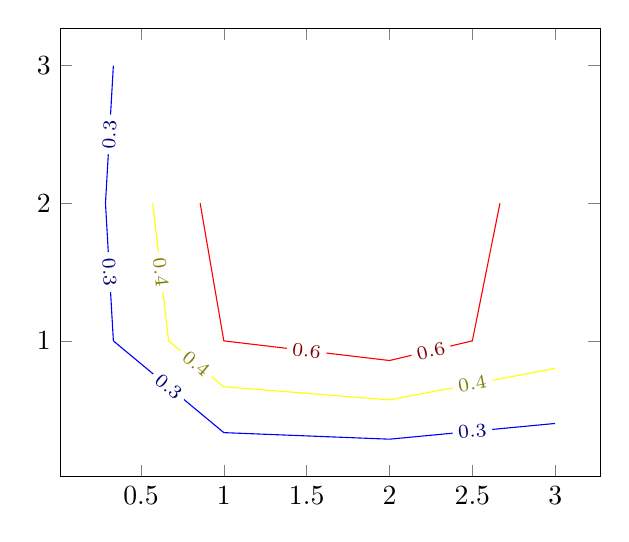
\begin{tikzpicture}
                \begin{axis}
                    \addplot[%
                        contour prepared,%
                        contour prepared format=matlab%
                    ] table { 
                        % (0.2,6) ==> contour `0.2' (x), 5 points follow (y): 
                        0.3000000e+00 6.0000000e+00 
                        3.0000000e+00 4.0000000e-01 
                        2.0000000e+00 2.8571429e-01 
                        1.0000000e+00 3.3333333e-01 
                        3.3333333e-01 1.0000000e+00 
                        2.8571429e-01 2.0000000e+00
                        3.3333333e-01 3.0000000e+00                         
                        % (0.4,5) ==> contour `0.4', consists of 5 points 
                        4.0000000e-01 5.0000000e+00 
                        3.0000000e+00 8.0000000e-01 
                        2.0000000e+00 5.7142857e-01 
                        1.0000000e+00 6.6666667e-01 
                        6.6666667e-01 1.0000000e+00 
                        5.7142857e-01 2.0000000e+00 
                        % (0.6,6) ==> contour `0.6', has 6 points 
                        6.0000000e-01 6.0000000e+00 
                        2.6666667e+00 2.0000000e+00 
                        2.5000000e+00 1.0000000e+00 
                        2.0000000e+00 8.5714286e-01 
                        1.0000000e+00 1.0000000e+00 
                        1.0000000e+00 1.0000000e+00 
                        8.5714286e-01 2.0000000e+00 
                    }; 
                \end{axis} 
            \end{tikzpicture}
        \end{figure}



        \begin{figure}[!hbt]
            \begin{tikzpicture}
                \begin{axis}
                    \addplot3[
                        mesh/rows=4,
                        mesh/num points=4,
                        contour gnuplot={
                            number=4,
                            % cdata should not be affected by z filter:
                            output point meta=rawz,
                            labels=false,
                        }
                    ] table [x index={1}, y index={2}, z index={3},col sep=comma] { 
                    1,-6.2832,-6.2832,0.74038,
                    2,-6.2832,-6.1563,0.74997,
                    3,-6.2832,-6.0293,0.75982,
                    4,-6.2832,-5.9024,0.76986,
                    }; 
                \end{axis} 
            \end{tikzpicture}
        \end{figure}